\begin{question}
\noindent A space mission archivist is cataloguing star-chart overlays. Shape $M$ represents a scanned constellation marker, and shape $M'$ represents the same marker found on an older, mirrored chart fragment. Shape $M'$ is the image of shape $M$ under a single reflection.

\begin{center}
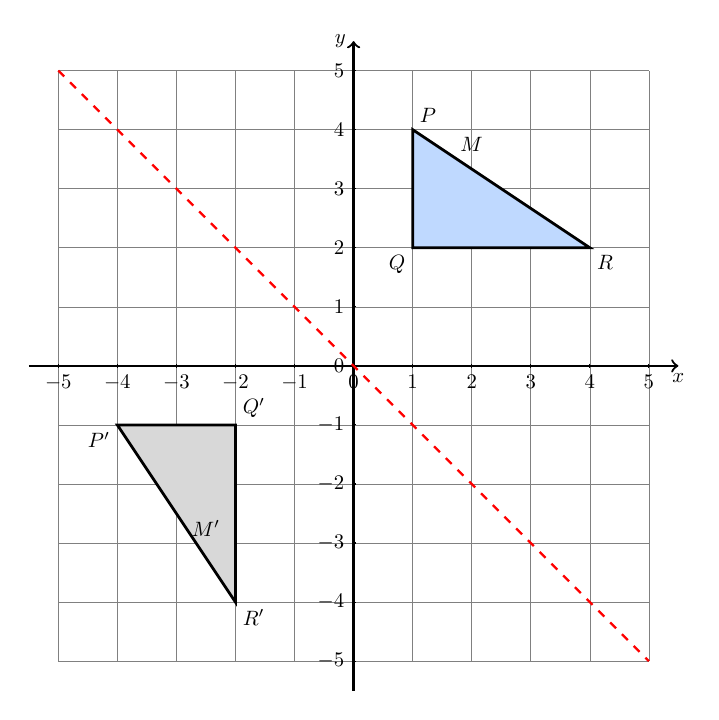
\begin{tikzpicture}[scale=0.75, transform shape]
    \def\axisLimit{5}

    \definecolor{borderColour}{HTML}{000000}
    \definecolor{fillColourM}{HTML}{BFD9FF}
    \definecolor{fillColourMp}{HTML}{D8D8D8}

    % Draw grid
    \draw[step=1cm,gray,very thin] (-\axisLimit,-\axisLimit) grid (\axisLimit,\axisLimit);

    % Draw axes
    \draw[thick,->] (-\axisLimit-0.5,0) -- (\axisLimit+0.5,0) node[anchor=north] {$x$};
    \draw[thick,->] (0,-\axisLimit-0.5) -- (0,\axisLimit+0.5) node[anchor=east] {$y$};

    % Label x-axis and y-axis
    \foreach \x in {-\axisLimit,...,\axisLimit}
        \draw (\x cm,1pt) -- (\x cm,-1pt) node[anchor=north] {$\x$};
    \foreach \y in {-\axisLimit,...,\axisLimit}
        \draw (1pt,\y cm) -- (-1pt,\y cm) node[anchor=east] {$\y$};

    % Mirror line y = -x
    \draw[thick, dashed, red] (-\axisLimit,\axisLimit) -- (\axisLimit,-\axisLimit);

    % Shape M: vertices (1,4), (1,2), (4,2)
    \coordinate (A) at (1,4);
    \coordinate (B) at (1,2);
    \coordinate (C) at (4,2);
    \filldraw[fill=fillColourM, draw=borderColour, line width=1pt] (A) -- (B) -- (C) -- cycle;
    \node[above right] at (A) {$P$};
    \node[below left] at (B) {$Q$};
    \node[below right] at (C) {$R$};
    \node[above] at (2,3.5) {$M$};

    % Shape M': reflection of M in y = -x
    % (x,y) -> (-y,-x)
    \coordinate (Ap) at (-4,-1);
    \coordinate (Bp) at (-2,-1);
    \coordinate (Cp) at (-2,-4);
    \filldraw[fill=fillColourMp, draw=borderColour, line width=1pt] (Ap) -- (Bp) -- (Cp) -- cycle;
    \node[below left] at (Ap) {$P'$};
    \node[above right] at (Bp) {$Q'$};
    \node[below right] at (Cp) {$R'$};
    \node[below] at (-2.5,-2.5) {$M'$};

\end{tikzpicture}
\end{center}

\noindent Describe fully the single transformation that maps shape $M$ onto shape $M'$.

\vspace{4cm}

\begin{flushright}
    \answerlines{2}{2}
\end{flushright}
\end{question}
